\documentclass[11pt,a4paper]{article}
\input{report/CE587_HW2_Style.sty}
\graphicspath{{./}{figures/}}
\begin{document}
\hypersetup{pageanchor=false}
\begin{titlepage}
  \thispagestyle{empty}
  \begin{flushright}{\large 11 November 2026\par}\end{flushright}
  \vspace*{0.5cm}
  \begin{center}
    
\includegraphics[width=0.42\textwidth]{metu_logo.jpg}\par
    \vspace{0.7cm}
    {\huge CE587 Homework 2\par}
    \vspace{0.3cm}
    {\Large Structural Optimization\par}
    \vspace{0.45cm}
    {\Large Fall Semester 2026--2027\par}
  \end{center}
  \vspace{1.0cm}
  \noindent
  \begin{minipage}[t]{0.48\textwidth}
    \raggedright
    {\Large\textbf{Submitted By}\par}
    \vspace{0.3cm}
    {\large Imran Shahriar\par}
    \vspace{0.2cm}
    {\large 2735835\par}
    \vspace{0.2cm}
    {\large MSc. in Structural Engineering\par}
  \end{minipage}\hfill
  \begin{minipage}[t]{0.48\textwidth}
    \raggedleft
    {\Large\textbf{Submitted To}\par}
    \vspace{0.3cm}
    {\large Prof. Dr. O\u{g}uzhan Hasan\c{c}ebi\par}
    \vspace{0.2cm}
    {\large Department of Civil Engineering\par}
    \vspace{0.2cm}
    {\large Middle East Technical University\par}
  \end{minipage}
  \vfill
  \begin{center}
    {\large Project files and source code}\par
    \vspace{0.15cm}
    \href{https://github.com/ImranMETU/CE587_Assignment2}{github.com/ImranMETU/CE587\_Assignment2}
  \end{center}
\end{titlepage}
\hypersetup{pageanchor=true}
\setcounter{page}{1}

\section{Introduction and problem definition}
\subsection{Design variables, objective and design space}
The design vector is $\bm x=(x_1,x_2)^T$, where $x_1$ and $x_2$ are
the horizontal and vertical displacements of the free truss joint, measured
in metres. Positive directions are rightward and downward, respectively.
The scalar objective is the total potential energy $f(\bm x)$ in joules,
which combines the elastic strain energy and the work of the applied load.
Minimizing it gives the equilibrium displacements for the supplied model.

The assignment is treated as unconstrained optimization. The supplied
objective is defined over $\bm x\in\mathbb R^2$, and no additional equality
or inequality constraints are imposed. Part (a) specifies the plotting
window $0<x_1<1$ m and $0<x_2<0.1$ m. These ranges define the contour
view. Numerical trial points may leave that window.

The geometry, material properties and applied load define the physical
problem. Part (h) examines numerical settings, including the starting point,
line-search width, stopping tolerance and damping parameters. The reported
sensitivity runs keep the physical inputs fixed so that each method solves
the same potential-energy problem.

\subsection{Mathematical formulation}
The free joint moves horizontally by $x_1$ (positive rightward) and vertically by
$x_2$ (positive downward). Each bar has length $s=\sqrt{(l/2)^2+h^2}$
with span $l=1.5$ m and height $h=4.0$ m. The material and loading data
are $E=207$ GPa, $A=10^{-5}$ m$^2$, $P=10^4$ N and $\theta=30^\circ$.
The potential energy is
\begin{align}
 f(\bm x)&=a x_1^2+b x_2^2-q_1 x_1-q_2 x_2,\\
 a&=\frac{EA}{s}\left(\frac{l}{2s}\right)^2,\\
 b&=\frac{EA}{s}\left(\frac{h}{s}\right)^2,\\
 q_1&=P\cos\theta,\qquad q_2=P\sin\theta.
\end{align}
Numerically, $s=4.069705$ m, $a=17274.4423$ N/m, $b=491361.9144$ N/m,
$q_1=8660.2540$ N and $q_2=5000$ N.

\clearpage
\subsection{Design space and graphical solution (parts a--b)}
Figure~\ref{fig:design} shows contours on the prescribed window.
In the magnified view, read the left and right extrema of the innermost
contour at about $0.248$ and $0.253$ m and the bottom and top extrema
at about $0.0046$ and $0.0056$ m. The midpoint of each pair estimates the
center. To the precision supported by the plot, this gives
$(0.251,0.0051)$ m, with reading precision of roughly $0.001$ m
horizontally and $0.0001$ m vertically. The ratio $b/a=28.44$ makes the contours narrower in the vertical
displacement direction in physical coordinates.
\begin{figure}[H]
\centering
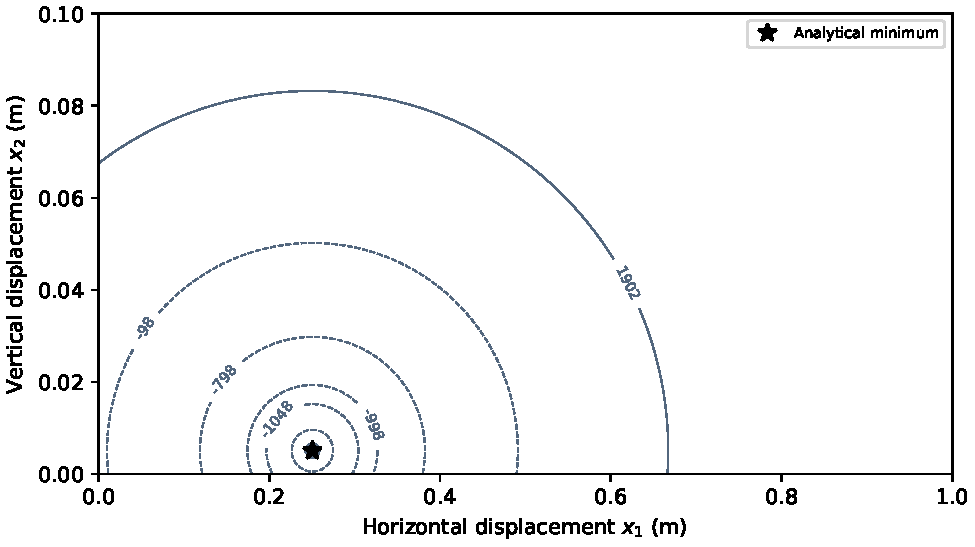
\includegraphics[width=.93\textwidth]{design_space.pdf}
\caption{Potential-energy contours in joules over the prescribed design space.}
\label{fig:design}
\end{figure}

\clearpage
\begin{figure}[H]
\centering
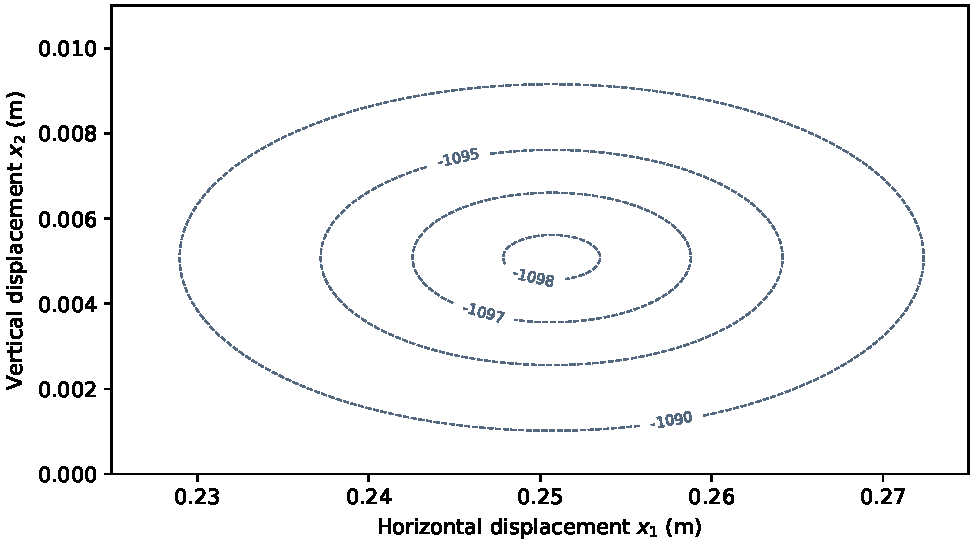
\includegraphics[width=.85\textwidth]{graphical.pdf}
\caption{Magnified contours in joules for estimating the center from opposite extrema.}
\end{figure}
\clearpage
\subsection{Analytical solution (part c)}
The calculation can be reproduced by hand as follows. Each bar has length
\[
s=\sqrt{0.75^2+4.0^2}=4.0697051490\ \mathrm m,
\qquad EA=(207\times10^9)(10^{-5})=2.07\times10^6\ \mathrm N.
\]
Using this length in the coefficients of the supplied energy equation gives
\begin{align*}
a&=\frac{EA}{s}\left(\frac{l}{2s}\right)^2=17274.4423\ \mathrm{N/m},\\
b&=\frac{EA}{s}\left(\frac{h}{s}\right)^2=491361.9144\ \mathrm{N/m},\\
q_1&=P\cos30^\circ=8660.2540\ \mathrm N,\qquad
q_2=P\sin30^\circ=5000\ \mathrm N.
\end{align*}
The numerical objective, with displacements in metres and energy in joules, is
\[
\begin{split}
f(x_1,x_2)={}&17274.4423x_1^2+491361.9144x_2^2\\
&-8660.2540x_1-5000x_2.
\end{split}
\]
Differentiate with respect to each displacement and set the derivatives to zero:
\begin{align*}
\frac{\partial f}{\partial x_1}&=34548.8846x_1-8660.2540=0,\\
\frac{\partial f}{\partial x_2}&=982723.8289x_2-5000=0.
\end{align*}
Solving these two linear equations gives
\[
x_1^*=\frac{q_1}{2a}=\frac{8660.2540}{34548.8846},\qquad
x_2^*=\frac{q_2}{2b}=\frac{5000}{982723.8289}.
\]
All calculations retain full precision internally. The displayed coefficients
are rounded. The second derivatives form the Hessian
\[
H=\begin{bmatrix}34548.8846&0\\0&982723.8289\end{bmatrix}\ \mathrm{N/m}.
\]
Its leading principal minors satisfy $H_{11}>0$ and
$\det H=H_{11}H_{22}>0$. Thus the Hessian is positive definite and the
stationary point is the unique global minimum. Substituting the resulting
displacements in the original objective gives
\[
 \boxed{\bm x^*=(0.2506666752,\,0.0050878994)^T\ \mathrm{m}},
 \qquad f^*=-1098.13829172\ \mathrm{J}.
\]
The free joint therefore moves approximately $250.667$ mm rightward and
$5.088$ mm downward. The minimum lies within the prescribed plotting window.

\clearpage
\subsection{Numerical implementation (parts d--f)}
With $\delta_i=0.01x_i$ and $D_i^{\pm}=f(\bm x\pm\delta_i\bm e_i)-f(\bm x)$,
the central stencils are
\[
 g_i=\frac{D_i^+-D_i^-}{2\delta_i},\qquad
 H_{ii}=\frac{D_i^++D_i^-}{\delta_i^2}.
\]
The four-point mixed stencil cancels identically because the quadratic is
separable. The implementations compute $D_i^{\pm}$ directly from the
quadratic increment to preserve precision near equilibrium. When a coordinate
is exactly zero, its relative stencil vanishes. In that case a 1 m reference
scale supplies the nonzero perturbation $\delta_i=0.01$ m at the baseline
stencil factor. At the initial
point, $\bm g=(-5205.37,\,4827.24)^T$ N.

\paragraph{Steepest descent (d).} Set $\bm p=-\bm g$ and update
$\bm x\leftarrow\bm x+\alpha\bm p$. With the baseline interval width,
the final candidate comparison selects $\alpha=0$ on the first iteration.
The starting point is therefore reported as stalled. After 14 halvings,
the final interval is $[0,2^{-14}]$. Its smallest positive candidate
is $2^{-15}\approx3.05\times10^{-5}$, larger than twice the line minimum,
so zero gives a lower energy than either positive candidate. The extended
run retains the gradient tolerance, uses width $10^{-13}$ and allows 400
updates. It converges at update 290 to $(0.2506666750,0.0050878994)$ m
with residual $8.81\times10^{-6}$ N.

\paragraph{Newton's method (e).} Solve $H\bm p=-\bm g$ and use the same
line search. The Newton direction is approximately $(0.1506666752,-0.0049121006)^T$
m at the start. The interval search selects the endpoint $\alpha=1$ and
the method reaches the minimum in one step.

\paragraph{Marquardt's method (f).} Solve $(H+\lambda I)\bm p=-\bm g$.
Accept a unit step when its energy decreases, then divide $\lambda$ by ten.
On rejection keep the current point and multiply $\lambda$ by ten. This
update rule is adopted here because the handout specifies only the initial
damping. The first trial point is approximately $(0.24643,0.005093)$ m.

\paragraph{Interval halving.} Start from $[0,1]$ and compare the midpoint
and two quarter points. Keep the half interval around the lowest candidate,
then compare the two endpoints and midpoint of the final interval.
For $f(\bm x+\alpha\bm p)=f(\bm x)+L\alpha+Q\alpha^2$, the comparisons
use distance to $-L/(2Q)$, which orders the trial energies without cancellation.
The first steepest-descent line minimum is $\alpha\approx2.11\times10^{-6}$.

\paragraph{Stopping test.} Use $\|\bm g\|_2\le10^{-5}$ N and an iteration
cap of 200 in the baseline runs. The extended and zero-start steepest-descent
runs allow 400 iterations, and the loose-tolerance run uses $10^{-2}$ N.
An interval search that returns zero above the gradient tolerance
is classified as stalled. The plot boundaries define the graphical view.
The optimization steps may leave that window.

\clearpage
\subsection{Worked central differences for parts (d)--(f)}
At the common starting point $(0.1,0.01)$ m, the prescribed perturbations are
$\delta_1=0.001$ m and $\delta_2=0.0001$ m. Direct substitution in the
original potential energy gives the values below. Retaining extra digits
is necessary when subtracting nearly equal energy values.
\begin{table}[H]
\centering
\caption{Objective evaluations for the initial central-difference stencil.}
\begin{tabular}{rrr}
\toprule
$x_1$ (m)&$x_2$ (m)&$f$ (J)\\
\midrule
0.100&0.0100&$-694.144789297752$\\
0.101&0.0100&$-699.332880432427$\\
0.099&0.0100&$-688.922149278469$\\
0.100&0.0101&$-693.657151849739$\\
0.100&0.0099&$-694.622599507476$\\
0.101&0.0101&$-698.845242984414$\\
0.101&0.0099&$-699.810690642151$\\
0.099&0.0101&$-688.434511830456$\\
0.099&0.0099&$-689.399959488193$\\
\bottomrule
\end{tabular}
\end{table}
The gradient components follow from the two opposite evaluations in
each coordinate:
\begin{align*}
g_1&\approx\frac{-699.332880432427-(-688.922149278469)}{0.002}
=-5205.365577\ \mathrm N,\\
g_2&\approx\frac{-693.657151849739-(-694.622599507476)}{0.0002}
=4827.238289\ \mathrm N.
\end{align*}
The diagonal second derivatives are
\begin{align*}
H_{11}&\approx
\frac{-699.332880432427-2(-694.144789297752)-688.922149278469}{(0.001)^2}\\
&=34548.8846\ \mathrm{N/m},\\
H_{22}&\approx
\frac{-693.657151849739-2(-694.144789297752)-694.622599507476}{(0.0001)^2}\\
&=982723.8289\ \mathrm{N/m}.
\end{align*}
The mixed stencil is
\[
H_{12}\approx
\frac{f_{++}-f_{+-}-f_{-+}+f_{--}}{4\delta_1\delta_2}\approx0,
\]
where the signs indicate the two coordinate perturbations. The mixed
derivative is exactly zero for this separable quadratic. Thus
$\|\bm g^{(0)}\|_2=7099.159$ N and the diagonal Hessian supplies the
curvatures for Newton and Marquardt. At every subsequent iterate, recompute
the perturbations and the central differences using the current coordinates.

\clearpage
\subsection{Worked steepest-descent and Newton updates}
\paragraph{Steepest descent, part (d).}
The direction and trial point are
\[
\bm p=-\bm g=
\begin{bmatrix}5205.365577\\-4827.238289\end{bmatrix},
\qquad
\bm x(\alpha)=
\begin{bmatrix}0.1+5205.365577\alpha\\0.01-4827.238289\alpha\end{bmatrix}.
\]
The direct line search starts on $[0,1]$. At each round it evaluates the
left quarter point, midpoint and right quarter point with the original
objective, retains the half containing the lowest value, and returns the
final interval midpoint once its width is below $10^{-4}$. The exact line
minimum is $\alpha_*=2.1143863\times10^{-6}$, far smaller than the first
returned midpoint. After 14 rounds the interval is
$[0,6.10352\times10^{-5}]$ and the returned midpoint is
$\alpha=3.05176\times10^{-5}$. Direct evaluation gives
$f(\bm x^{(1)})\approx8867.23$ J, up from $-694.14$ J. The method therefore
accepts an uphill step. Repeating the stated procedure leads to overflow;
the first nonfinite state occurs at iteration 103, so this run diverges
before the limit $M=200$.

As a separate direction-scaling case, use
$\bm p=-\bm g/\|\bm g\|_2$ with the same $[0,1]$ interval, width and cap.
Here $\alpha$ has units of metres. This removes the huge scale of the raw
gradient direction and produces a useful path, but at iteration 200 the
run is still above tolerance, with $\|\bm g\|_2\approx18.57$ N. It is
reported as capped, not converged. The finer, extended runs are parameter
sensitivity cases and are not substituted for the prescribed baseline.

\paragraph{Newton, part (e).}
Solving $H\bm p=-\bm g$ gives
\[
p_1=\frac{5205.365577}{34548.8846}=0.1506666752\ \mathrm m,
\qquad
p_2=\frac{-4827.238289}{982723.8289}=-0.0049121006\ \mathrm m.
\]
The direct interval search returns $\alpha=1-2^{-15}$. After the first
update, the next Newton direction has norm $4.60\times10^{-6}$ m, below
the lecture step tolerance. The point is $(0.2506620773,0.0050880493)$ m
and the residual gradient is $0.21665$ N.

\clearpage
\subsection{Worked Marquardt update and displacement paths}
\paragraph{Marquardt, part (f).}
At $\lambda_0=1000$ N/m, the first trial is
$\bm x=(0.24642838,\,0.00509289)^T$ m. Its directly evaluated energy
is $-1097.827976$ J, below the starting value. Accept it and set
$\lambda=500$ N/m. On each rejection retain the current point and double
$\lambda$; on each acceptance halve it. With this lecture-note rule and
direct objective comparisons, the run reaches the gradient tolerance after
eight trials, with five accepted updates. Three trials near the solution
are rejected when the directly evaluated energy fails the strict decrease test.
\begin{table}[H]
\centering
\caption{Selected direct-evaluation Marquardt iterates.}
\begin{tabular}{rrrr}
\toprule
$k$&$x_1$ (m)&$x_2$ (m)&$\|\bm g\|_2$ (N)\\
\midrule
0&0.1000000000&0.0100000000&$7099.159$\\
1&0.2464283798&0.0050928928&$146.511$\\
2&0.2506062126&0.0050879020&$2.089$\\
3&0.2506662409&0.0050878994&$1.501\times10^{-2}$\\
4&0.2506666737&0.0050878994&$5.410\times10^{-5}$\\
8&0.2506666752&0.0050878994&$7.718\times10^{-7}$\\
\bottomrule
\end{tabular}
\end{table}
\begin{figure}[H]
\centering
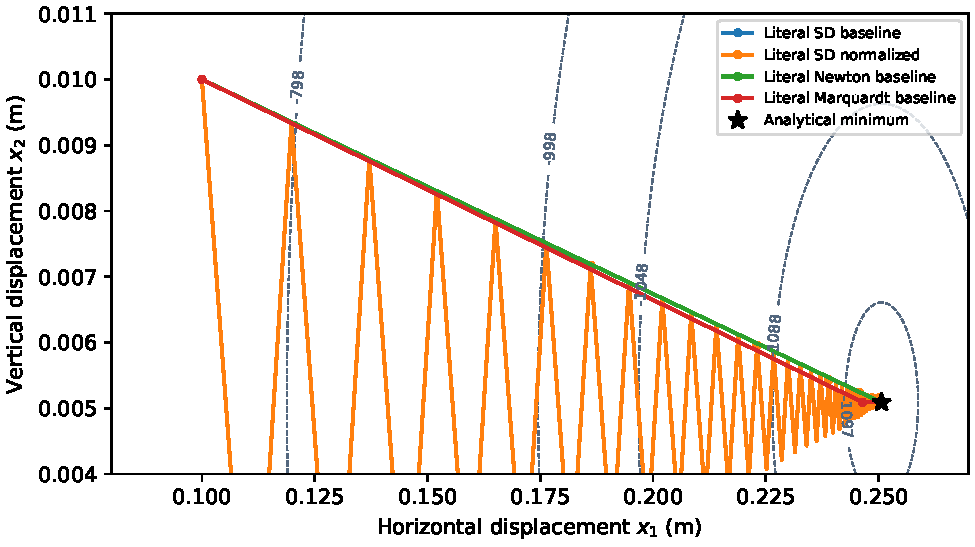
\includegraphics[width=.85\textwidth]{baseline_detail.pdf}
\caption{Magnified baseline displacement paths for parts (d)--(f). Newton meets the lecture step test after one update, while Marquardt meets
the gradient test after eight trials. The normalized
steepest-descent path is shown here; the unnormalized direct run diverges.
The full-window paths appear in the baseline comparison.}
\end{figure}
For part (c), the analytical point is marked on the full contour plot and
the positive-definite Hessian proves the minimum. The displacement paths
provide the iteration diagrams requested for parts (d)--(f).


\clearpage
\section{Convergence and parameter sensitivity}
\subsection{Baseline comparison (part g)}
All methods start at $(0.1,0.01)$ m. The line-search width is $10^{-4}$ for
steepest descent and Newton, and the initial damping is $10^3$ N/m for
Marquardt. Figure~\ref{fig:base} shows the three paths.
\begin{figure}[H]
\centering
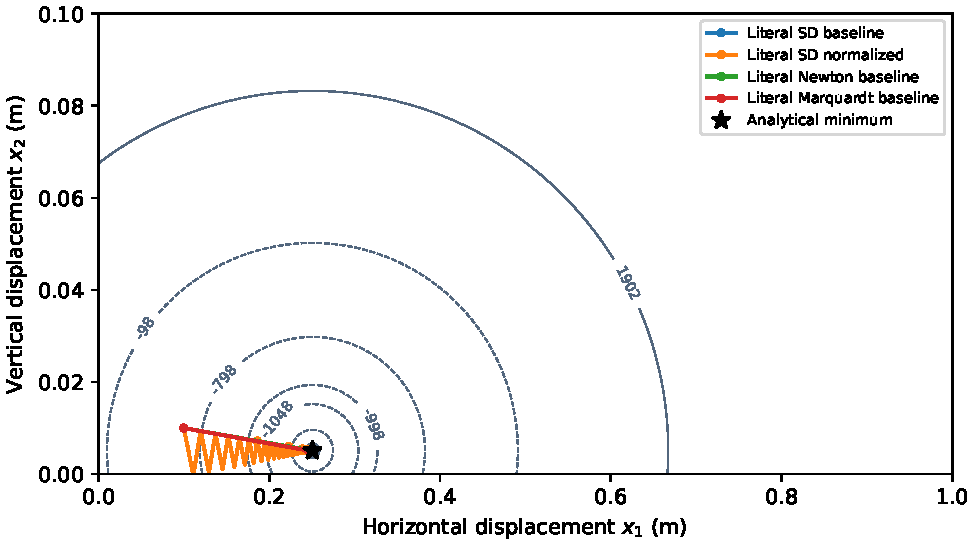
\includegraphics[width=.95\textwidth]{baseline.pdf}
\caption{Baseline iterates on the prescribed design space. The steepest-descent path consists of the initial point.}
\label{fig:base}
\end{figure}

\begin{table}[H]
\centering
\caption{Convergence with stabilized arithmetic for the baseline and selected sensitivity runs.}
\label{tab:convergence}
\begin{tabular}{llrrrr}
\toprule
Method & Setting & Updates & Trials$^\dagger$ & $\|\bm g\|_2$ (N) & Status\\
\midrule
Steepest descent & Baseline & 0 & 49 & $7.10\times10^3$ & Stalled\\
Newton & Baseline & 1 & 63 & $<10^{-8}$ & Converged\\
Marquardt & Baseline & 4 & 49 & $<10^{-8}$ & Converged\\
\midrule
Steepest descent & Width $10^{-13}$ & 200 & 27804 & $5.12\times10^{-3}$ & Cap\\
Steepest descent & Extended & 290 & 40314 & $8.81\times10^{-6}$ & Converged\\
Newton & Width $10^{-13}$ & 1 & 153 & $<10^{-8}$ & Converged\\
Marquardt & $\lambda_0=10^5$ & 6 & 69 & $<10^{-8}$ & Converged\\
\bottomrule
\end{tabular}
\end{table}
\noindent{\small $^\dagger$Estimated objective-sample counts use four central-difference
samples per steepest-descent update and nine for the full Hessian stencil,
three trial samples per interval-halving round plus three final candidates,
and one trial per Marquardt update. The derivative increments and line-search
comparisons are simplified analytically in the implementation. These counts
are a transparent work estimate, not measured runtime or an exact count of
all arithmetic operations.}

By update count, Newton is fastest at one update and Marquardt follows at four.
The steepest-descent baseline makes no update because its line search selects
zero; it must be reported as stalled rather than as a converged fast run.
For a broader efficiency comparison, the estimated sample count favors
Marquardt over Newton in this implementation, 49 versus 63. This does not
make Marquardt universally more efficient: both counts depend on the declared
stencil and search conventions, and the Hessian here is especially cheap to
solve because it is diagonal. The extended steepest-descent run changes both
the line-search width and iteration cap, so it illustrates attainable
convergence rather than isolating one parameter effect.

\clearpage
\subsection{Sensitivity runs and verification (part h)}
The first three rows in the convergence table are one-setting comparisons
against their named baseline: the line-search width is tightened for steepest descent and Newton,
and only $\lambda_0$ changes in the Marquardt run. All other settings carry
over. With the tighter search, steepest descent reaches
$(0.2506665666,0.0050879030)$ m at iteration 200, about $1.09\times10^{-7}$ m
from the solution. The gradient remains above the stopping threshold. Newton
still needs one update, with more interval comparisons. Larger initial
Marquardt damping makes the first update smaller and raises the iteration
count from four to six.

\paragraph{Steepest-descent rate.} The Hessian condition number is
$\kappa=b/a=28.44$. For a positive-definite quadratic with exact line
minimization, the worst-case per-step contraction in the Hessian norm
$\|e\|_H=(e^THe)^{1/2}$, where $e=x-x^*$, is
$(\kappa-1)/(\kappa+1)=0.9321$. For the stabilized extended run the
geometric mean contraction from iterations 100 to 290 is
$(\|e_{290}\|_H/\|e_{100}\|_H)^{1/190}=0.9317$.
\begin{figure}[H]
\centering
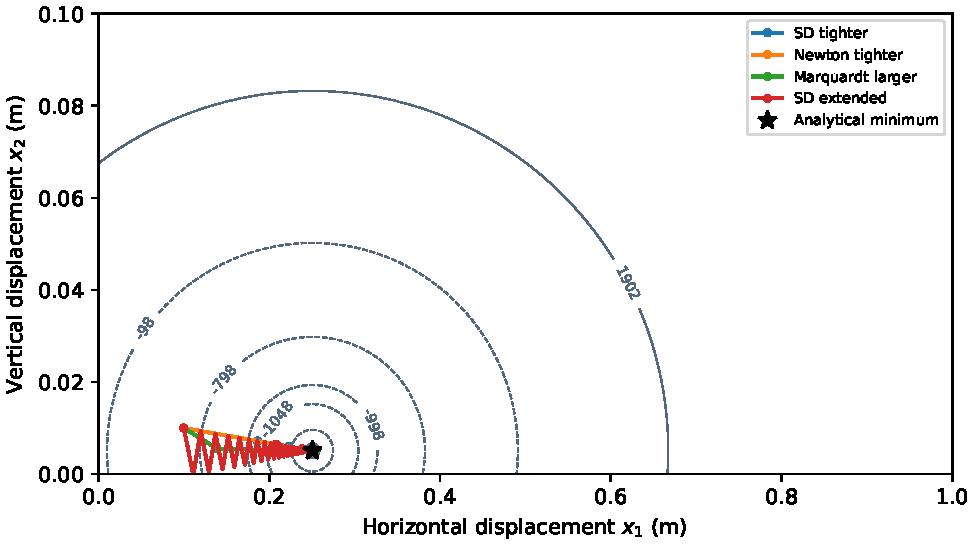
\includegraphics[width=.86\textwidth]{sensitivity.pdf}
\caption{Sensitivity iterates in the assigned plotting window.}
\end{figure}
\begin{figure}[H]
\centering
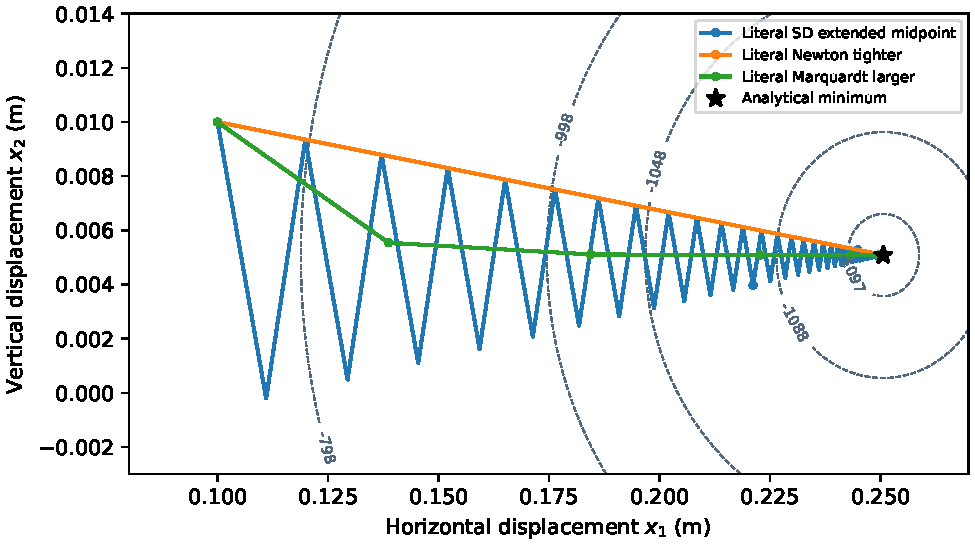
\includegraphics[width=.86\textwidth]{detail.pdf}
\caption{Detail of the same paths, including negative $x_2$ values visited by steepest descent.}
\end{figure}

\clearpage
\subsection{Additional sensitivity runs}
\begin{table}[H]
\centering
\caption{One-setting changes from the named reference run.}
\begin{tabular}{llrr}
\toprule
Reference run & Setting changed & Updates & Final gradient (N)\\
\midrule
SD tighter & Cap 400 & 290 & $8.81\times10^{-6}$\\
SD extended & Start $(0,0.01)$ m & 220 & $8.65\times10^{-6}$\\
Newton baseline & Stencil factor $10^{-4}$ & 1 & $1.42\times10^{-8}$\\
Marquardt baseline & Damping factor 2 & 5 & $9.77\times10^{-8}$\\
SD tighter & Gradient tolerance $10^{-2}$ N & 192 & $9.01\times10^{-3}$\\
\bottomrule
\end{tabular}
\end{table}
The changed starting point changes the mixture of directional errors and
the subsequent steepest-descent path. A looser gradient tolerance saves
updates at the expense of equilibrium accuracy. Central differences are
exact for this quadratic in exact arithmetic, so the smaller stencil changes
the Newton residual through rounding. The factor of two decreases damping
more slowly after acceptance, adding one update in the stabilized run.

\paragraph{Newton line-search check.} Python held the derivative stencil
fixed and varied the energy comparison and final candidate policy separately.
Both raw objective values and stabilized comparisons gave one update with
the best of the final endpoints and midpoint. Returning the midpoint gave
two updates with stabilized comparisons and seven with raw values. Thus both
the endpoint policy and rounding can affect the trace near equilibrium.

\paragraph{Direct objective evaluation.} Additional Python runs compute the
central differences from raw objective values, including the four-point
mixed stencil, and compare raw objective values in the line search or
Marquardt acceptance test. The stalled steepest-descent baseline persists.
Table~\ref{tab:arithmetic} shows that the iteration counts can change when
rounding affects the order of nearby trial energies. In particular, the
direct Marquardt run with a factor of two rejects three trials whose computed
energies fail the strict decrease test. The direct counts also depend on
the evaluation order of the floating-point expression for $f$.

\begin{table}[H]
\centering
\caption{Iterations with stabilized and direct objective arithmetic in Python.
Marquardt counts include rejected trials.}
\label{tab:arithmetic}
\begin{tabular}{lrr}
\toprule
Case & Stabilized & Direct\\
\midrule
Steepest descent, extended & 290 & 275\\
Newton, best final candidate & 1 & 1\\
Newton, final midpoint & 2 & 6\\
Marquardt, damping factor 2 & 5 & 8\\
\bottomrule
\end{tabular}
\end{table}

\clearpage
\subsection{Discussion and method selection}
\paragraph{Steepest descent.}
With the suggested line-search width of $10^{-4}$, the final candidate
comparison selects a zero step even though the starting gradient norm
is about $7{,}099$ N. Tightening the search allows progress, but the
unequal curvatures produce a zigzag path. The tighter run is within
$1.09\times10^{-7}$ m of the analytical solution after 200 iterations,
with a gradient norm still above tolerance. Allowing more iterations
gives convergence at iteration 290 with stabilized arithmetic and 275
with direct objective evaluation.

\paragraph{Newton's method.}
The energy is quadratic and the Hessian is constant and positive definite.
Since $\bm g=H(\bm x-\bm x^*)$, the Newton direction points directly
from the current iterate to the minimum. The baseline line search
accepts the full step, giving convergence in one iteration with either
arithmetic implementation. Tightening the search adds comparisons
while leaving the iteration count at one.

\paragraph{Marquardt's method.}
Adding $\lambda I$ to the Hessian reduces the step, particularly along
the softer horizontal direction. The baseline takes four accepted
steps and reaches the same minimum. Increasing the initial damping
from $10^3$ to $10^5$ N/m reduces the first step and raises the count to
six. Under the equivalent-sample convention in Table~\ref{tab:convergence}, the baseline
uses 49 samples versus Newton's 63 because it avoids interval halving.

\paragraph{Method selected.}
Newton's method is preferred for this truss. It reaches the analytical
minimum in the fewest iterations, and the diagonal Hessian makes the
direction calculation inexpensive. Marquardt uses fewer equivalent
samples under the chosen accounting convention. Those counts describe
the stencil and search work, so the recommendation rests on Newton's
one-step convergence and inexpensive Hessian solve.

\clearpage
\subsection{Iteration checkpoints and settings}
\begin{table}[H]
\centering
\caption{Selected iterates for the three algorithms.}
\begin{tabular}{lrrrr}
\toprule
Run & $k$ & $x_1$ (m) & $x_2$ (m) & $\|\bm g\|_2$ (N)\\
\midrule
Common start & 0 & 0.100000000 & 0.010000000 & $7.10\times10^3$\\
Newton baseline & 1 & 0.250666675 & 0.005087899 & $4.39\times10^{-11}$\\
Marquardt baseline & 1 & 0.246428380 & 0.005092893 & $1.47\times10^2$\\
Marquardt baseline & 4 & 0.250666675 & 0.005087899 & $3.54\times10^{-9}$\\
SD extended & 200 & 0.250666567 & 0.005087903 & $5.12\times10^{-3}$\\
SD extended & 290 & 0.250666675 & 0.005087899 & $8.81\times10^{-6}$\\
\bottomrule
\end{tabular}
\end{table}

The full per-iteration results, including each trial step and gradient,
are available in the CSV and workbook.

\clearpage
\subsection{Parameter list and sensitivity settings}
The problem definition and physical parameters are collected below.
The displacements are the quantities to be determined, and the objective
is the energy to be minimized.
\begin{table}[H]
\centering
\caption{Problem definition, physical inputs and design space.}
\begin{tabular}{p{0.26\textwidth}p{0.66\textwidth}}
\toprule
Quantity & Definition or value\\
\midrule
Design variables & $\bm x=(x_1,x_2)^T$ in m, positive rightward and downward\\
Objective & $\min_{\bm x}f(x_1,x_2)$, total potential energy in J\\
Constraints & No imposed equality or inequality constraints\\
Mathematical domain & $\bm x\in\mathbb R^2$ for the supplied objective\\
Contour design space & $0<x_1<1$ m and $0<x_2<0.1$ m\\
Material and section & $E=207\times10^9$ Pa, $A=10^{-5}$ m$^2$\\
Geometry & $l=1.5$ m, $h=4.0$ m\\
Applied load & $P=10^4$ N, $\theta=30^\circ$\\
Derived bar length & $s=\sqrt{(l/2)^2+h^2}=4.0697051490$ m\\
\bottomrule
\end{tabular}
\end{table}
The following numerical settings implement the baseline and part (h).
Each comparison changes the setting indicated in the sensitivity table,
relative to its named reference run. The 400-update runs and the finer
line search are explicitly identified as sensitivity settings.
\begin{table}[H]
\centering
\caption{Baseline numerical settings and sensitivity overrides.}
\begin{tabular}{lll}
\toprule
Parameter & Baseline & Overrides\\
\midrule
Starting displacements (m) & $(0.1,0.01)$ & $(0,0.01)$\\
Maximum updates & 200 & 400\\
Gradient tolerance (N) & $10^{-5}$ & $10^{-2}$\\
Relative stencil factor & $0.01$ & $10^{-4}$\\
Line-search interval & $[0,1]$ & \\
Line-search width & $10^{-4}$ & $10^{-13}$\\
Initial damping (N/m) & $10^3$ & $10^5$\\
Damping multiplier & 10 & 2\\
\bottomrule
\end{tabular}
\end{table}

\clearpage
\section{Calculation files and reproducibility}
The handout for CE587 Homework 2, Fall 2026--2027 supplies the geometry,
load, material properties, baseline numerical parameters and plotting window.
\begin{itemize}
 \item \texttt{solve\_hw2.py} generates the iteration CSV and six vector plots.
 \item \texttt{CE587\_HW2\_Validation.xlsx} computes the geometry, exact
 minimum, finite differences and eleven runs using worksheet formulas.
 Its Results sheet compares its final coordinates with the Python output.
 \item \texttt{python\_iterations.csv} records the Python states and termination
 reasons, including the Python-only direct objective and Newton line-search checks.
\end{itemize}
\small\noindent\textbf{Python--Excel consistency.} The 935 stabilized states match in count, status, damping and evaluation; steps differ by less than $10^{-10}$. Maximum coordinate, energy and gradient differences are $3.21\times10^{-8}$ m, $1.21\times10^{-4}$ J and $5.43\times10^{-3}$ N. Long SD traces amplify floating-point ties. Shared formulas make this a consistency check; the analytical and literal runs are separate checks.\normalsize

\end{document}
